\documentclass[../main.tex]{subfiles}
 
\begin{document}

\section{Thursday}

You luck out. You seem to have had a shift removed from your schedule. In the morning you help a studio responsible for virtual reality content production and distribution. You again find yourself putting VR headsets on people's heads and wiping them down for the next attendee. You're happy to kill downtime during the lulls in the last day's foot traffic by talking to the guy helping to run the booth. He is apparently freelancing for the production company who owns the music videos made for Bono that are preloaded on each of these headsets. The headsets are Sony Gear units, since they apparently come with higher end smartphones and thus will be the main target for the distribution of VR-related content, for now. This guy you are helping out graduated from UCLA recently with a degree in film; now he's working in a Venice, California office for a company called Within. He seems to have a a few good ideas and you talk at length about Louie C.K.'s new independently produced episodic content for \textit{Horace and Pete}. You have no idea how this guy is going to crack into the industry, and you feel starting in VR is possibly a bad move. Unfortunately, you don't make it over to see the highly praised 360 Google Spotlight Story \textit{Pearl} just a few booths away. While you have been less than impressed with much of the VR stuff that made its way to SIGGRAPH, \textit{Pearl} apparently gets the story part right, making use of VR to further the story without relying on the gimmick as so many other booths have done.

With a few hours left before setting off for the beach, you hope to hear some more technical talks. When you wander up to the third floor of the Convention Center to pop into Ballroom B for a talk on meshes and fields, you last only 5 minutes before you must excuse yourself. The speaker is dreadful and as with your experience during the Vulcan talk, you cannot get a foothold any point during the presentation. You walk next door to Ballroom C for a presentation titled \textit{Mass Effect: New Earth --- A 4D Holographic Adventure}. The panel doesn't exactly seem to be full of engineers. After a few minutes of marketing baloney with words like "heavy tech" thrown around, you again excuse yourself to look through the bookstore before heading back downstairs. Oh well, you feel like you have gotten a lot out of SIGGRAPH and now shift gears to gathering anyone you can for Huntington Beach.


\begin{figure}[h!]
	\centering
	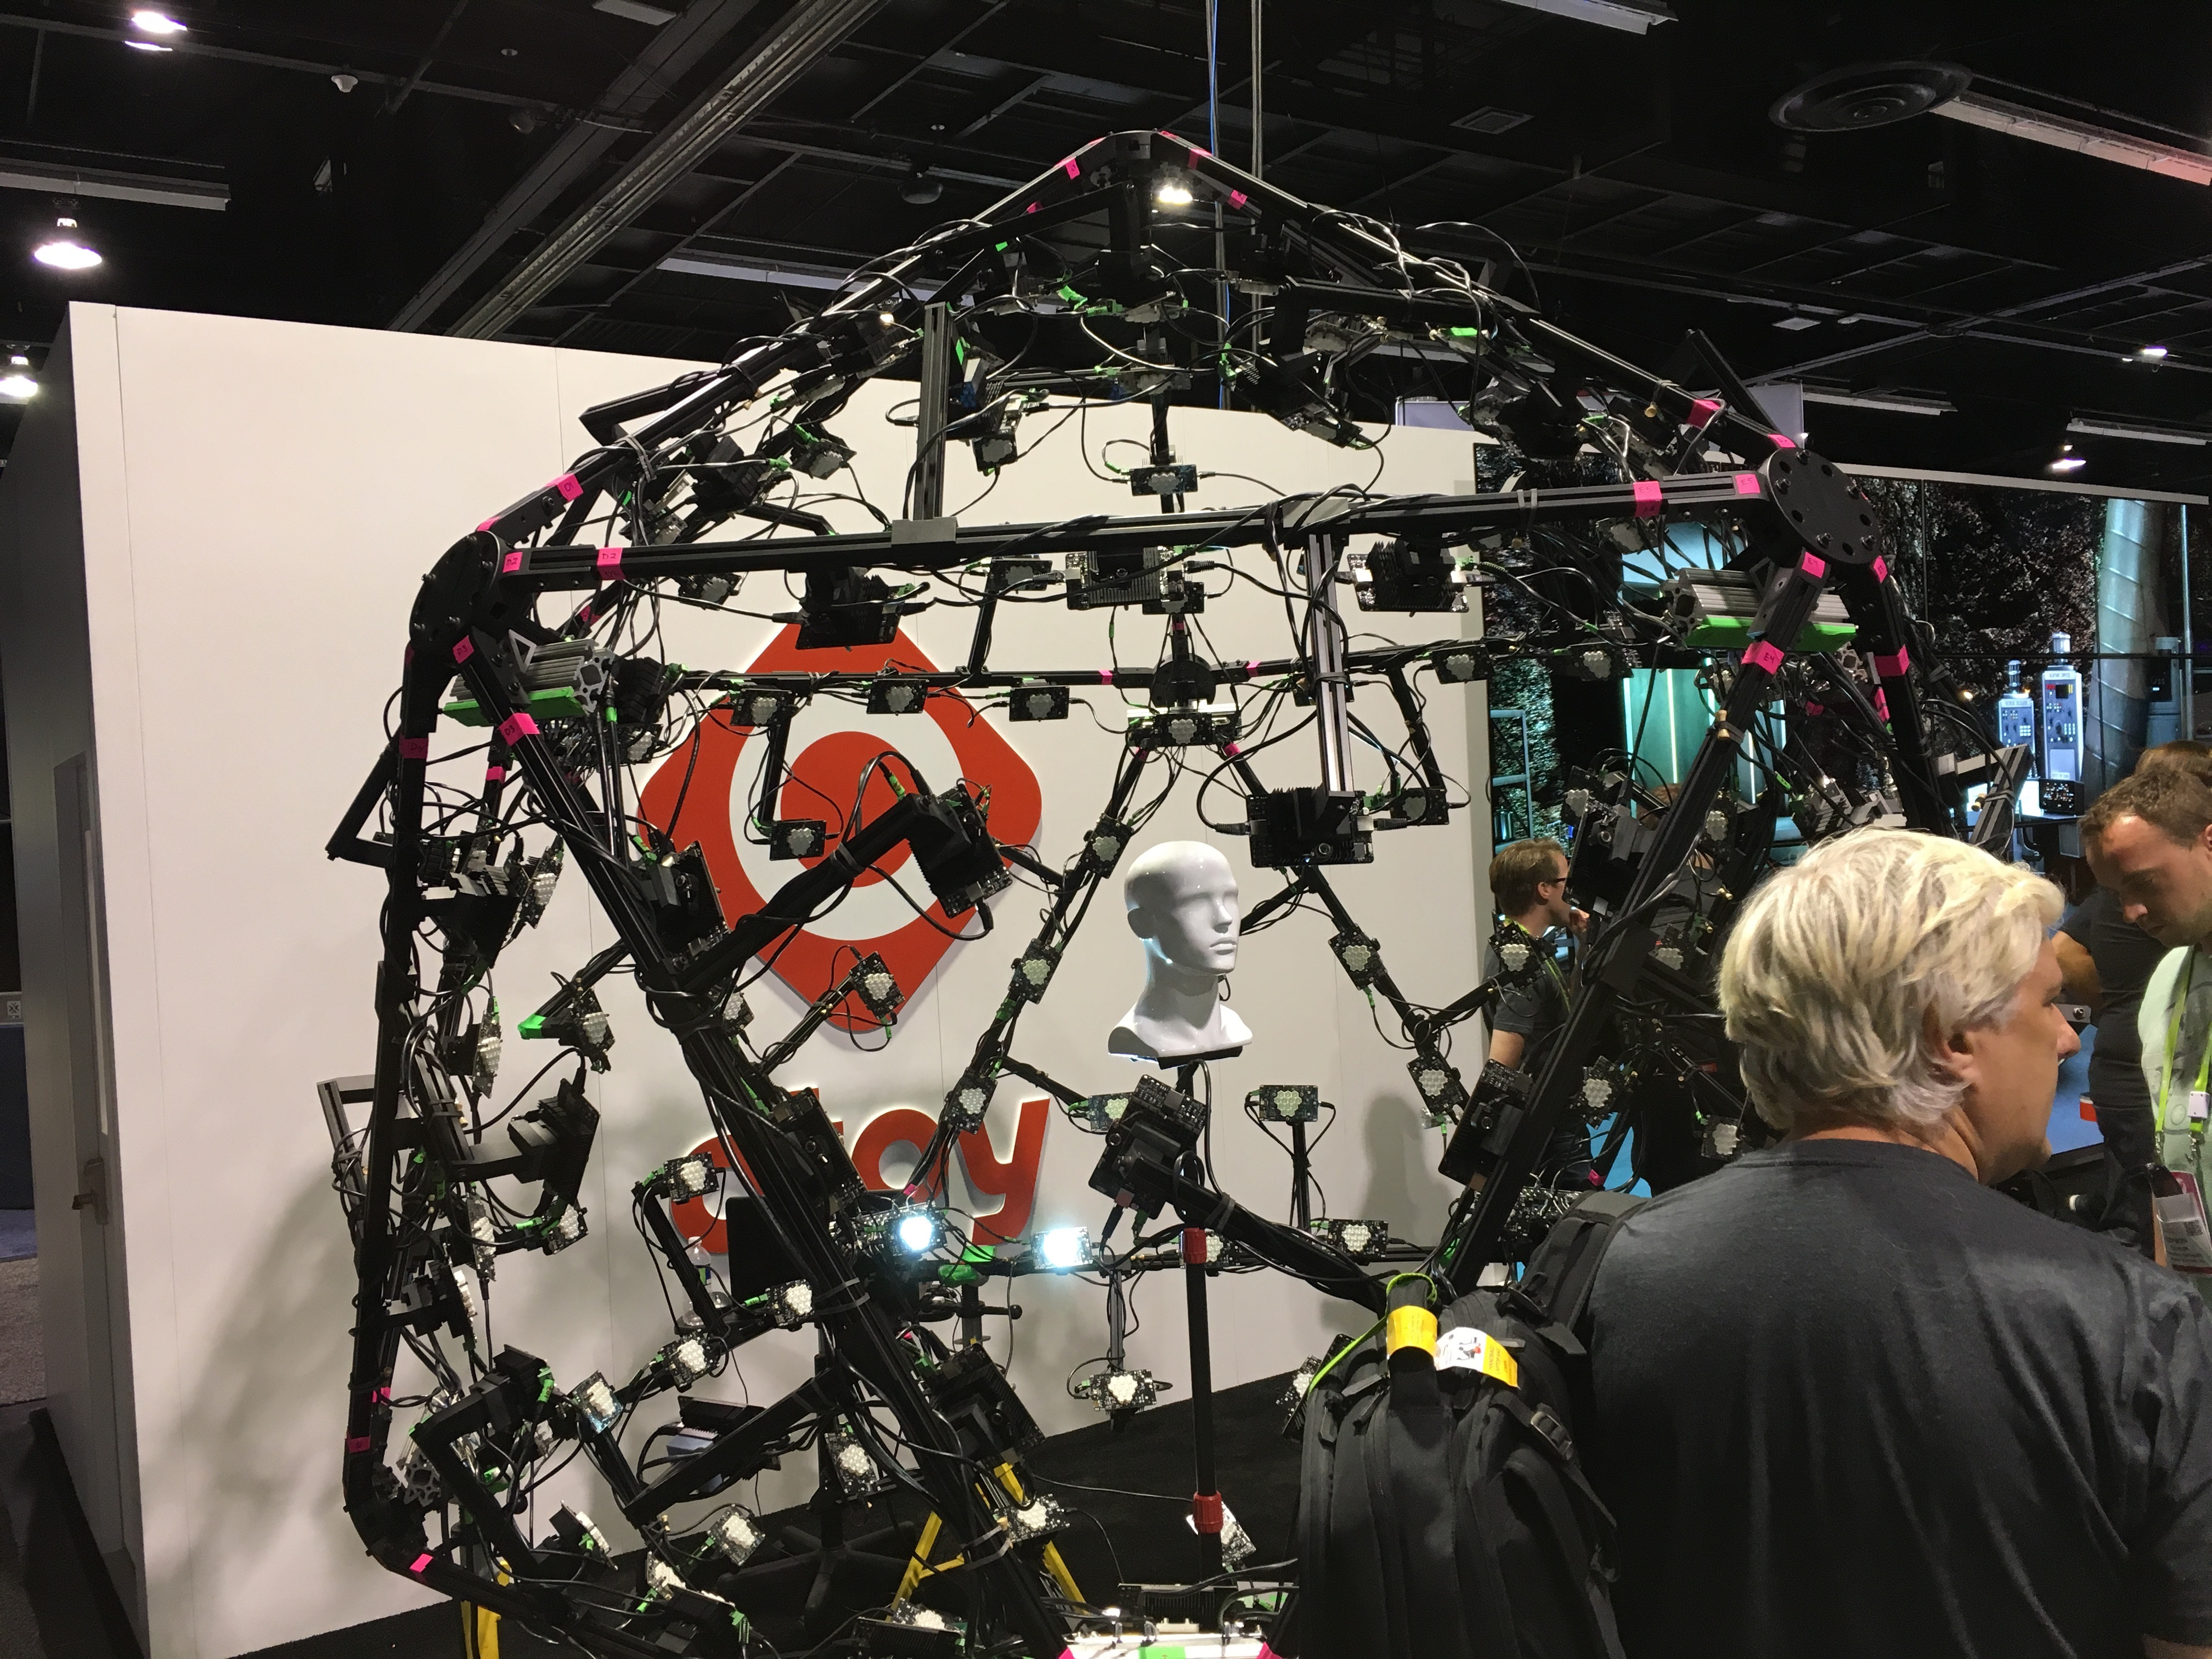
\includegraphics[width=\textwidth]{lighting}
	\caption*{This machine is designed to recreate complex lighting situations for live filming.}
\end{figure}


Since some of your friends are still finishing their shifts during the final hours of SIGGRAPH, you wonder through Exhibition Hall before all of the vendors close for the day. You check out the a NVIDIA demo where you walk into a trailer housing a high powered desktop computer and a HTC Vive setup (two, in fact, as this demo is made to immerse two paticipants in the same world). You try out an automotive application which allows you to use a controller in your hand to select options which are immediately reflected in the configuration of a car parked in front of you. What you see in your virtual world is a large garage and a shiny car sitting on the expoxied shop floor. You are encouraged by the gentlemen from Autodesk standing in the room with you to walk over to the car and kneel down inside it. You can lie down on the floor and look at the underbelly of the car, get up, and walk around it. Your physical controller allows you to point at several green orbs in this world as a means of flicking between various viewpoints, where selecting a viewpoint is a matter of shooting a red beam at an orb as if you were using a small laser pointer. Because of the cameras positioned in the NVIDEA booth which track your head in high fidelity, you are afforded a VR experience at an entirely different level of immersion than what is offered by Occulus and the Sony Gear (which utilizes a modest Android phone). You ask some questions and are put off by the overly aggressive sales pitch of the Autodesk marketing guy. He explains that he comes from the automotive industry, and you believe him. Later, months after SIGGRAPH is over, you will come to realize the guy you spoke to is Paul Schmucker, co-host and producer of Everyday Driver, which you watch for car reviews on YouTube from time to time.

\begin{figure}[h!]
	\centering
	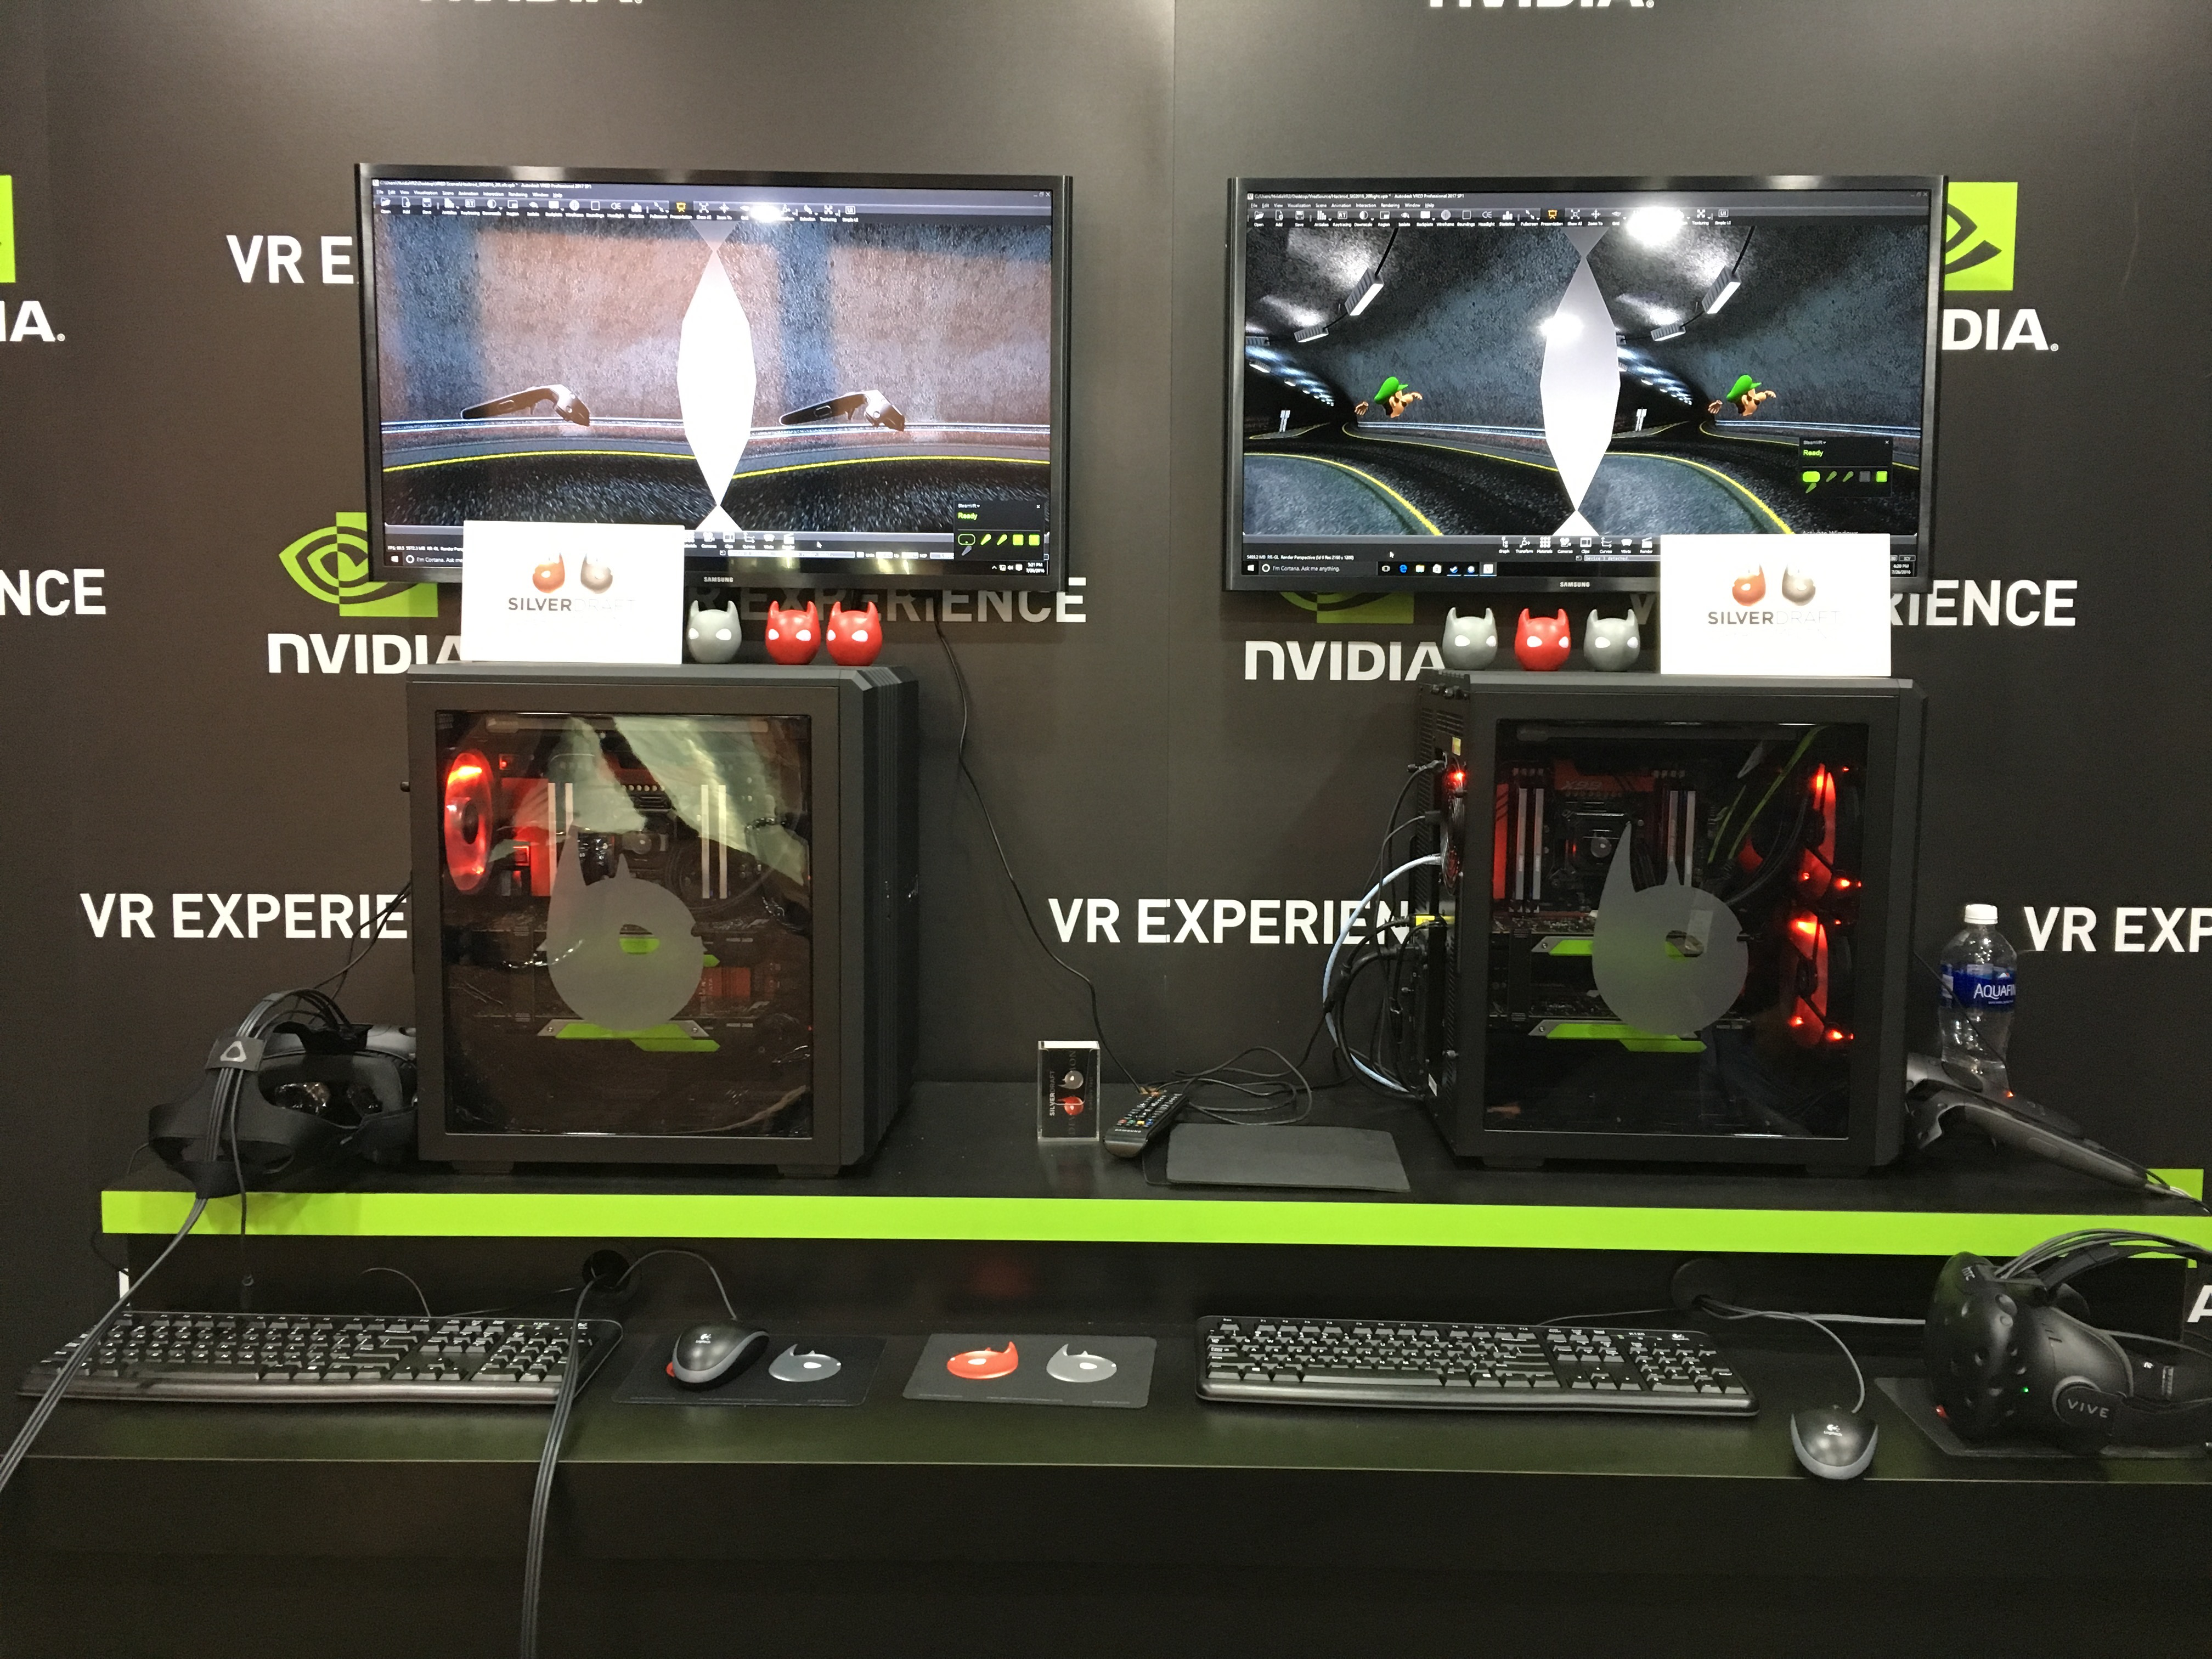
\includegraphics[width=\textwidth]{htc_vive}
	\caption*{The HTC Vive. Brought to you by NVIDIA and Autodesk.}
\end{figure}

The wrap-up for SIGGRPAH 2016 takes the form of a SV raffle held in the room adjacent to the SV office on the second floor of the Conventon Center. You all gather into chairs and eye the tables at the front of the room with mugs, hats, Pixar teapots, signed posters, thousands of dollars worth of graphics cards, and other miscellaneous goodies. A guest speaker who worked at the Jet Propulsion Laboratory speaks to all of you and encourages you to make the best of such an incredible field. He is joining the Student Volunteer Program Chair, Christian Wittorf, along with several other committee members in thanking all of you seated in the room for your contribution. Everyone is getting anxious as the prizes sit unclaimed at the front of the room. Finally, the names are called and you win a nice \textit{SIGGRAPH 2016} hat and a poster for Disney's upcoming animated shot \textit{Inner Workings}, which you will hang near your desk at work. After the raffle prizes are distributed, you also score a Pixar teapot from the extras given out for folks who missed out on the RenderMan party. Diede would have given one to you, but he was saving his second for his brother. These teapots are highly sought after (or so it seems), and yours will sit proudly on your desk at work. Your group decides to stick together for the rest of the day as you walk out of the Convention Center and begin to make preparations for the trip to Huntington Beach.

After collecting people one by one at their hotels, it is Jen, Diede, and another girl named Ambar who pack into a comically small Uber car with you and head towards the ocean. After a stop at Johnny Rockets, \textit{because this is America}, you all find a spot in the sand some 20 paces from the water. You haven't been to the beach in a while, and neither has Diede. You have all arrived later than you had hoped to, but you catch the tail end of the golden hour of light as Jen, Diede, and you take off running into the breaking waves. Ambar guards the belongings, wanting to be near the water, but not \textit{in} the water. Shivering, you all return to your burgers, pour out Heineken into little red Solo cups, and toast to SIGGRAPH 2016.

\begin{figure}[h!]
	\centering
	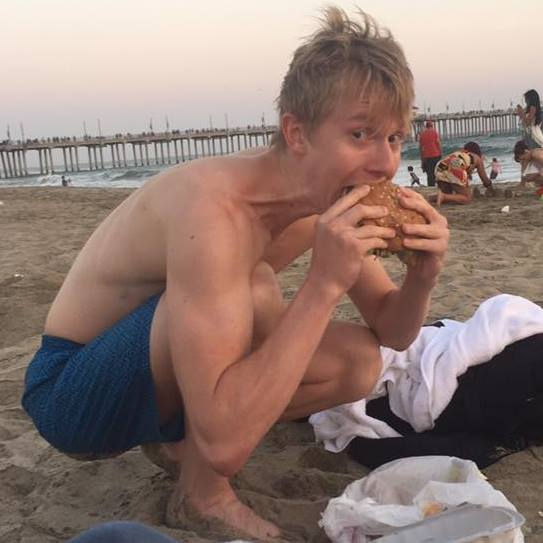
\includegraphics[width=0.6\textwidth]{beach}
	\caption*{Huntington Beach.}
\end{figure}

At some point in the evening, you pose to the group the following question: "What are you really excited about working on when you get back?" Jen describes a vision for an art project that she hopes to complete. You also encourage everyone to go around and share their favorite memories of the past week. You say that yours was seeing the evolution of set design for \textit{Finding Dory}. Stories of college are shared, with Diede at one point describing the fascinating a capella groups at the school he just graduated from in the Netherlands. He regales the group with stories of extreme and hilarious situations members would be placed in which might be described as \textit{hazing}. The night winds down. You all pack back into an Uber and make your way back to a hotel. With the windows of the driver's Prius open and the cool air hitting your face, you watch the lights of neighborhoods and industrial districts wash past while the others nod off in the backseat alongside you. It seems like a little over half an hour passes as you drive along the now empty highways.

Back at Jen's hotel you all say goodbye and wish each other well, encouraging everyone to stay in touch and not be afraid to reach out on Facebook. The week is over, but there's no reason you can't keep your world small by keeping tabs on Diede and his work and seeing where Jen and Ambar land in the coming year. You hug, shake Diede's hand, as he half-jokingly insists, and make your way back to your host so that you can pack your things. You will be tired when you wake up early for your flight,  but you did nearly everything you could have hoped to do at your first SIGGRAPH. You learned some new things, received encouragement from people like Philip Nemec, made friends, told stories, and came away humbled by the incredible talent of your fellow SVs. You also literally got your feet wet. SIGGRAPH pulls you out of your bubble and reminds you of the beauty of making things and showing them to other people. You are thankful for the opportunity to attend SIGGRAPH, which would not have happened if it were not for Chris Tralie and all of the other mentors you had at Duke.

So off you go, to make things, program, and write. There is so much to learn and at least a few new books and recent papers are waiting for you to read them. What you have seen at SIGGRAPH has helped remind you that what you want to do will require more math. It will require more \textit{of a lot of things}. You do not yet know many of the things that you will need to understand in order to create elegant software or write what you hope you can write or tell the story you think you will tell. As Chris Tralie once told you, \textit{you should not let not knowing everything stop you from doing anything}. There's not a whole lot stopping you from using the resources you already have available to in order to continue your education, to do math. It is easy to become overwhelmed by things you can see at SIGGRAPH, but that's okay.

You hope to not be distracted by trends, and you want to work hard to make something that is truly elegant. You have seen great work at SIGGRAPH 2016 and you had the chance to meet the people who go back when all is said and done to keep doing great work. You look forward to SIGGRAPH 2017 and other events like it because while not every aspect of SIGGRAPH may be worth the price of admission, there seem to be enough surprises and fortuitous encounters to warrant getting on a plane and spending a few days milling about a convention center in a hot touristy destination like Anaheim. Some of SIGGRAPH is silly, sure, but it is still a gathering of talented people and therefore worth attending, especially as a student volunteer, if you have the slightest interest in making dreams a reality through computer graphics. You just have to put on blinders and tune out the commercials to get the most of this event.

\end{document}